\section{Eksperimen}
\label{sec:eksperimen}

\subsection{Pengujian Gerakan}

\begin{figure} [ht]
  \centering
  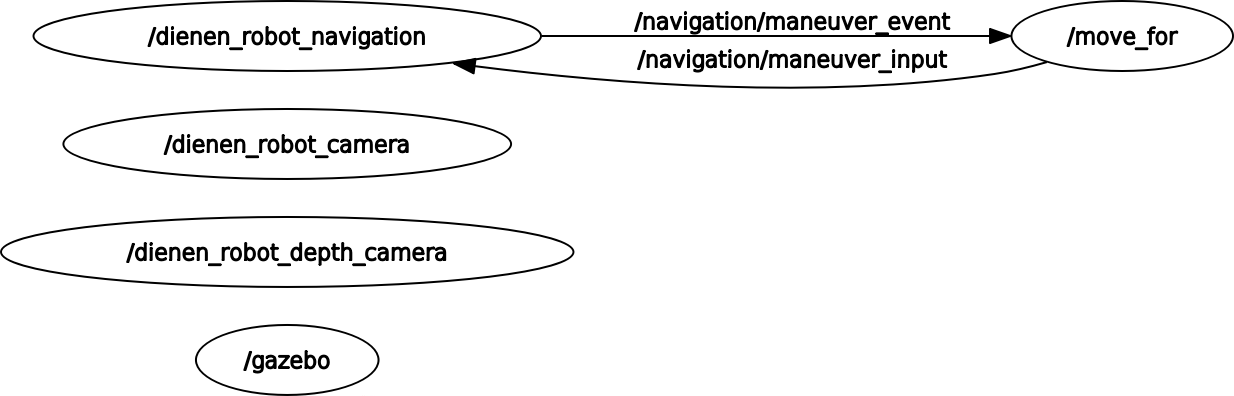
\includegraphics[scale=0.25]{gambar/nodeujigerak.png}
  \caption{Skema node pengujian gerakan linier.}
  \label{fig:nodeujigerak}
\end{figure}

Pengujian gerakan dilakukan dengan menjalankan node \lstinline{move_for} sebagai \emph{node behavior} yang akan memerintahkan robot untuk bergerak dengan kecepatan tertentu selama kurun waktu tertentu.
Seperti yang terlihat pada Gambar \ref{fig:nodeujigerak}, di simulasi, node \lstinline{move_for} akan terhubung dengan node \lstinline{dienen_robot_navigation} untuk mengatur kecepatan dari robot yang ada di simulasi melalui topic \lstinline{/navigation/maneuverinput}.
Sedangkan untuk pengujian pada robot fisik, peran dari node \lstinline{dienen_robot_navigation} yang mengatur navigasi pada robot virtual akan digantikan oleh node \lstinline{navigation} yang mengatur navigasi yang ada pada robot fisik.

\lipsum[1-5]
